\documentclass[conference]{IEEEtran}
\IEEEoverridecommandlockouts
% The preceding line is only needed to identify funding in the first footnote. If that is unneeded, please comment it out.
\usepackage{cite}
\usepackage{amsmath,amssymb,amsfonts}
\usepackage{algorithmic}
\usepackage{graphicx}
\usepackage{textcomp}
\usepackage{xcolor}
\usepackage{mathtools}
\usepackage{subfigure}

\def\BibTeX{{\rm B\kern-.05em{\sc i\kern-.025em b}\kern-.08em
    T\kern-.1667em\lower.7ex\hbox{E}\kern-.125emX}}
\begin{document}

\title{Orientation Tracking and Panorama Generation\\

}

\author{\IEEEauthorblockN{1\textsuperscript{st} Pengxi Zeng}
    La Jolla, CA \\
    p2zeng@ucsd.edu}


\maketitle

\begin{abstract}
    This is a report regarding orientation tracking and corresponding panorama generation. It mainly discussed how to
    define the motion model and observation model and utilize the IMU measurements to optimize the rotation quaternions.
    Gradient descent is adopted as the main method for optimization and a combianation of projection-based and normalization-
    based optimization metrics are used to constrain the quaternions to space $\mathbb{H}_*$. The result turns out good for
    most datasets. Finally, the panorama is
    generated using sphere-cylinder projection by first transforming the spherical coordinates of each pixel of the picture from
    camera frame to world frame. The final outcome shows great consistency in space, also indicating good effects of the optimization
    for the quaternions.
\end{abstract}

\begin{IEEEkeywords}
    orientation tracking, panorama, gradient descent
\end{IEEEkeywords}

\section{Introduction}

If we want to precisely control the motion of the robots, it is very important that we first need to know how they move, which is
how to quatify the movement. In practice, the gyroscopes and accelerometers are usually adopted to get the measurements of the
motion of the body. In this report, we present a method to utilize the data collected by an IMU (the collection of a gyroscope and
a accelerometer) to regenerate the rotation matrix.


\section{Problem Formulation}
\subsection{Orientation Tracking}
Generally, we have two models to describe the realtion between the rotation quaternions and real measurements:

\begin{equation}
    \boldsymbol{q}_{t+1} = f(\boldsymbol{q}_t, \tau_t \omega_t) \coloneq \boldsymbol{q}_t \circ exp([0, \tau_t\omega_t/2]). \label{motion}
\end{equation}

\begin{equation}
    \boldsymbol{a}_t = h(\boldsymbol{q}_t) \coloneq \boldsymbol{q}_t^{-1} \circ [0, a_x, a_y, a_z] \circ q_t. \label{observation}
\end{equation}

The equations above are motion model \eqref{motion} and observation model \eqref{observation} respectively. Motion model mainly
describes how to calculate the rotation quaternion at the next moment rotating with a specific anguler velocity and time interval.
And observation model mainly describes the acceleration distribution in IMU frame. The measurements collected from IMU should match
with calculated results from the two models \eqref{motion}-\eqref{observation}. Thus, we could define two losses to decribe the
distance between the model and the measurement:

\begin{equation}
    loss_{motion} = \frac{1}{2}||2\text{log}(\boldsymbol{q}_{t+1}^{-1} \circ f(\boldsymbol{q}_t, \tau_t \omega_t))||_2^2 \label{lossMotion}
\end{equation}

\begin{equation}
    loss_{observ} = \frac{1}{2} || \boldsymbol{a}_t - h(\boldsymbol{q}_t) ||_2^2
\end{equation}

The loss related to the motion model indicates that we need future rotation quaternions to compute the loss. For the loss related
to observation model, considering that the body is assuming to be undergoing pure rotation, we could only take gravity into account,
which leads to $[a_x, a_y, a_z] = [0, 0, -g]$ in \eqref{observation}. The overall cost could be formulated as:
\begin{equation}
    \begin{aligned}
        c(\boldsymbol{q}_{1:T}) \coloneq \frac{1}{2}\sum\limits_{t=0}^{T-1}||2\text{log}(\boldsymbol{q}_{t+1}^{-1}
        \circ f(\boldsymbol{q}_t, \tau_t \omega_t))||_2^2 \\
        + \frac{1}{2} \sum\limits_{t=1}^{T}|| \boldsymbol{a}_t - h(\boldsymbol{q}_t) ||_2^2
    \end{aligned}
\end{equation}

Therefore, we could formulate this problem as how to minimize the overall cost $c(\boldsymbol{q}_{1:T})$. Also, we need to ensure
that the quaternions are valid, which means $||\boldsymbol{q}_t||_2 = 1$. We hence have a constrained optimization problem:
\begin{equation}
    \begin{aligned}
        \min\limits_{\boldsymbol{q}_{1:T}} c(\boldsymbol{q}_{1:T}) \\
        \text{s.t.} ||\boldsymbol{q}_t||_2 = 1,
    \end{aligned}
\end{equation}
where the initial value should be $\boldsymbol{q}_0 = [1, 0, 0, 0]$

\subsection{Panorama Generation}
As the body rotates, the camera carried by the robot is taking pictures of the room, resulting in a picture array $pic_{1:T}$.
Assuming each pixel of one picture is distributed over a unit sphere, with corresponding spherical coordinates $(1, \theta,
    \phi)$. We could adopt following steps to get the panorama.
\begin{itemize}
    \item Convert the spherical coordinates to Cartesian coordinates in camera frame;
    \item Convert Cartesian coordinates from camera frame to world frame
    \item Inscribe the sphere surface to cylinder surface, and unwrap the cylinder surface to rectanguler picture.
\end{itemize}


Therefore, we have set up general steps for a formulae of transforming a picture array to a picture:
\begin{equation}
    f: \mathbb{R}^{r \times c \times n} \rightarrow \mathbb{R}^{r \times c},
\end{equation}
where $r$ and $c$ stand for rows and columns and $n$ for the count of the pictures.


\section{Technical Approach}
\subsection{Orientation Tracking}
Since it is nearly not possible to find the closed solution to the problem, we adopt gradient descent to optimize the
quaternions step by step.

\textit{Optimization}:
For any quaternion $\boldsymbol{q}_t, \forall t \in [1, T]$, the optimization from step $k$ to $k+1$ could be formulated as:
\begin{equation}
    \begin{aligned}
        \boldsymbol{q}_t^{k+1} & = \boldsymbol{q}_t^{k} - \alpha \frac{\partial c(\boldsymbol{q}_{1:T})}
        {\partial \boldsymbol{q}_t^{k}} , \forall t \in [1, T]
    \end{aligned}
\end{equation}

However, if adopting this approach alone would lead to invalid quaternions ($\boldsymbol{q}_t \notin \mathbb{H}_*$). Thus, we need
validation step to modify the optimization step, in order to satisfy the constraint.

\textit{Validation}
There are two ways to achieve optimization validation. One is to directly adopt normalization, which is:
\begin{equation}
    \boldsymbol{q}_t^{k+1} = \frac{\boldsymbol{q}_t^{k} - \alpha \frac{\partial c(\boldsymbol{q}_{1:T})}
    {\partial \boldsymbol{q}_t^{k}}}{||\boldsymbol{q}_t^{k} - \alpha \frac{\partial c(\boldsymbol{q}_{1:T})}
    {\partial \boldsymbol{q}_t^{k}}||_2}.
\end{equation}
This approach mainly has two disadvantages, one is that $||\boldsymbol{q}_t^{k} - \alpha \frac{\partial c(\boldsymbol{q}_{1:T})}
    {\partial \boldsymbol{q}_t^{k}}||_2$ may equal to $0$, leading to sigularity.
The other is that the process could only cover part of the solution space,
losing possible solutions. Therefore, we have another approach, which is to project the gradient calculated in every optimization
step to tangent space and normalize the result. And then use the projection and the previous value to renew the $\boldsymbol{q}_t$:
\begin{equation}
    \boldsymbol{g}_t^k = \frac{\partial c(\boldsymbol{q}_{1:T})}{\partial \boldsymbol{q}_t^{k}},
\end{equation}
\begin{equation}
    \boldsymbol{h}_t^k = \boldsymbol{g}_t^k - (\boldsymbol{g}_t^k \cdot \boldsymbol{q}_t^k)\boldsymbol{q}_t^k,
\end{equation}
\begin{equation}
    \boldsymbol{n}_t^k = \boldsymbol{h}_t^k / ||\boldsymbol{h}_t^k||_2,
\end{equation}
\begin{equation}
    \boldsymbol{q}_t^{k+1} = \boldsymbol{q}_t^k\cos\phi_t^k + \boldsymbol{n}_t^k\sin\phi_t^k,
\end{equation}
where we need to optimize $\phi_t^k$ by adopting linear gradient search. In practice, we combine two methods to optimize $\boldsymbol{q}_t$,
which is to first use projection-based optimization in first few epochs and adopt normalization-based optimization in the last
few epochs.

\subsection{Panorama Generation}
To generate the panorama, the first step is to get the spherical coordinates in the camera frame for each pixel. The assumption
is that the pixels of the picture lies on a unit sphere. Given that the camera has a horizontal and vertical field of view with
angles $\frac{\pi}{3}$ and $\frac{\pi}{4}$ respectively, the azimuth angle $\phi$ and inclination $\theta$ of each pixel lies in
the range $-\frac{\pi}{6} \leq \phi \leq \frac{\pi}{6}$ and $\frac{3\pi}{8} \leq \theta \leq \frac{5\pi}{8}$. Then for a specific
pixel at $i$-th row and $j$-th column, the spherical coordinate should be defined as:
\begin{equation}
    r = 1
\end{equation}

\begin{equation}
    \phi = \frac{\pi}{6} - \frac{j}{\#cols} \frac{\pi}{3}
\end{equation}

\begin{equation}
    \theta = \frac{3\pi}{8} + \frac{i}{\#rows} \frac{\pi}{4}
\end{equation}

Then we convert the spherical coordinate to Cartesian coordinate by using the following formulae:
\begin{equation}
    x_{i, j} = \cos(\phi_{i, j})\sin(\theta_{i, j})
\end{equation}
\begin{equation}
    y_{i, j} = \sin(\phi_{i, j})\sin(\theta_{i, j})
\end{equation}
\begin{equation}
    z_{i, j} = \cos(\theta_{i, j})
\end{equation}

Notice that for every picture, the coordinate of a pixel at position $(i, j)$ is the same. We could
use a tensor to represent the coordinates of the picture take at time $t$ in the camera frame as:
$P_{t, c} \in \mathbb{R}^{r \times c \times 3}$.
Thus, given the rotation matrix $R_t$ and translation vector $\boldsymbol{p}_t$, we could convert the coordinates to
world frame as:
\begin{equation}
    P_{t, w}^T = R_t \times P_{t, c}^T + \boldsymbol{p}_t
\end{equation}

As long as the Cartesian coordinates of the pixels have been obtained, we could then obtain the spherical
coordinates in the world frame using:

\begin{equation}
    \phi_w = \arctan\frac{y_w}{x_w}
\end{equation}
\begin{equation}
    \theta_w = \arccos z_w
\end{equation}

Then we project the spherical coordinates to cylindrical coordinates by assigning the spherical azimuth to cylinder height
and inclination along the circumference. Thus for one pixel with the spherical coordinates as $(1, \theta, \phi)$, its position
in the panorama (interpreted as $(i_p, j_p)$-indexed) could be calculated as:
\begin{equation}
    i_p = \frac{\theta_w}{\pi} \#rows_p,
\end{equation}
\begin{equation}
    j_p = \frac{\phi_w + \pi}{2\pi} \#cols_p,
\end{equation}
in which we interpret the pixels with spherical coordinates $(1, 0, \phi)$ as the center line.

\subsection{Some More Details}
\textbf{The initialization of $\boldsymbol{q}_T$}: considering the fact that $\boldsymbol{q}_T$ is initialized using
motion model, the loss related to motion model is very small at first, and the gradient could become NAN. Thus, when
initializing $\boldsymbol{q}_T$, we added a small noise to it in order to make it bias from original value, so that
NAN would not appear at the start and could better train the model.

\textbf{Training}: when training the model, though we added a noise to $\boldsymbol{q}_T$ in initialization, the loss of
the motion model is still very small. To balance the two loss a little bit, we multiplied the motion loss by 10.

\textbf{Panorama}: when generating panorama, we changed the shape of the coordinates to $[3 \times (r \times c)]$ for
acceleration of the calculation.


\section{Results}
\subsection{Orientation Tracking}
From the results, we can find out that for most of the datasets, angles of Roll and Pitch match with real data realtively
well, but for Yaw, the shape of optimized results match with that of the real data, while the is a gap between them. One
guess is that the accumulation of the error in Yaw could not be well eliminated.

\subsection{Panorama}
From the results we can tell that the pictures have the consistency in space, e.g. the connection of the handrail.

\begin{figure}[htbp]
    \centering
    \subfigure[Roll for Dataset 1]{
        \begin{minipage}[t]{1\linewidth}
            \centering
            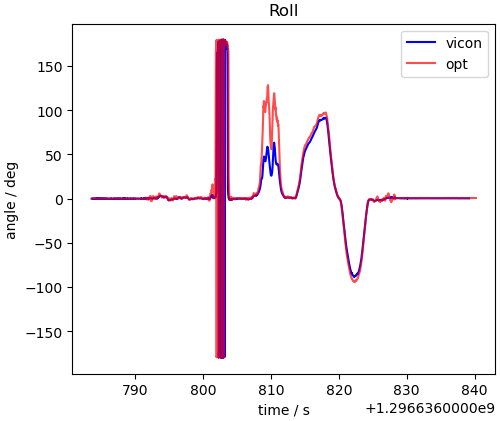
\includegraphics[width=2.5in]{../figs/Roll_1.png}
            % \caption{}
        \end{minipage}%
    }%

    \subfigure[Pitch for Dataset 1]{
        \begin{minipage}[t]{1\linewidth}
            \centering
            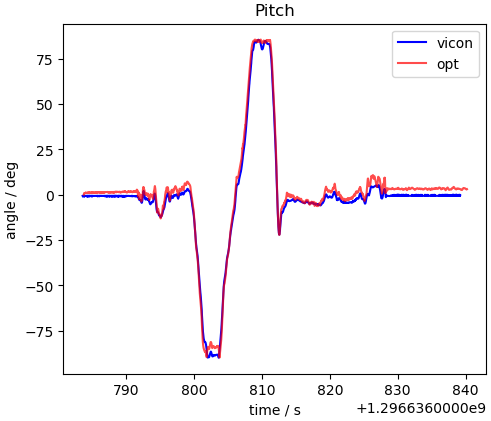
\includegraphics[width=2.5in]{../figs/Pitch_1.png}
            % \caption{}
        \end{minipage}
    }%

    \subfigure[Yaw for Dataset 1]{
        \begin{minipage}[t]{1\linewidth}
            \centering
            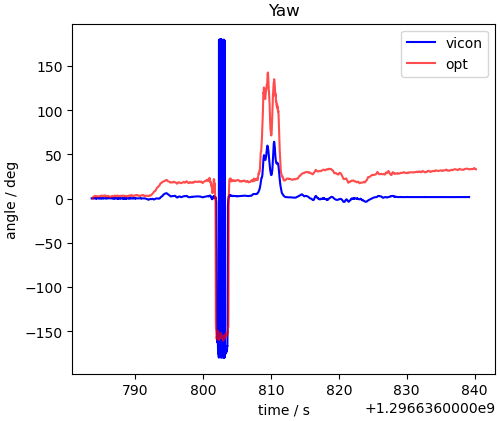
\includegraphics[width=2.5in]{../figs/Yaw_1.png}
            % \caption{}
        \end{minipage}
    }%

    \subfigure[Panorama for Dataset 1]{
        \begin{minipage}[t]{1\linewidth}
            \centering
            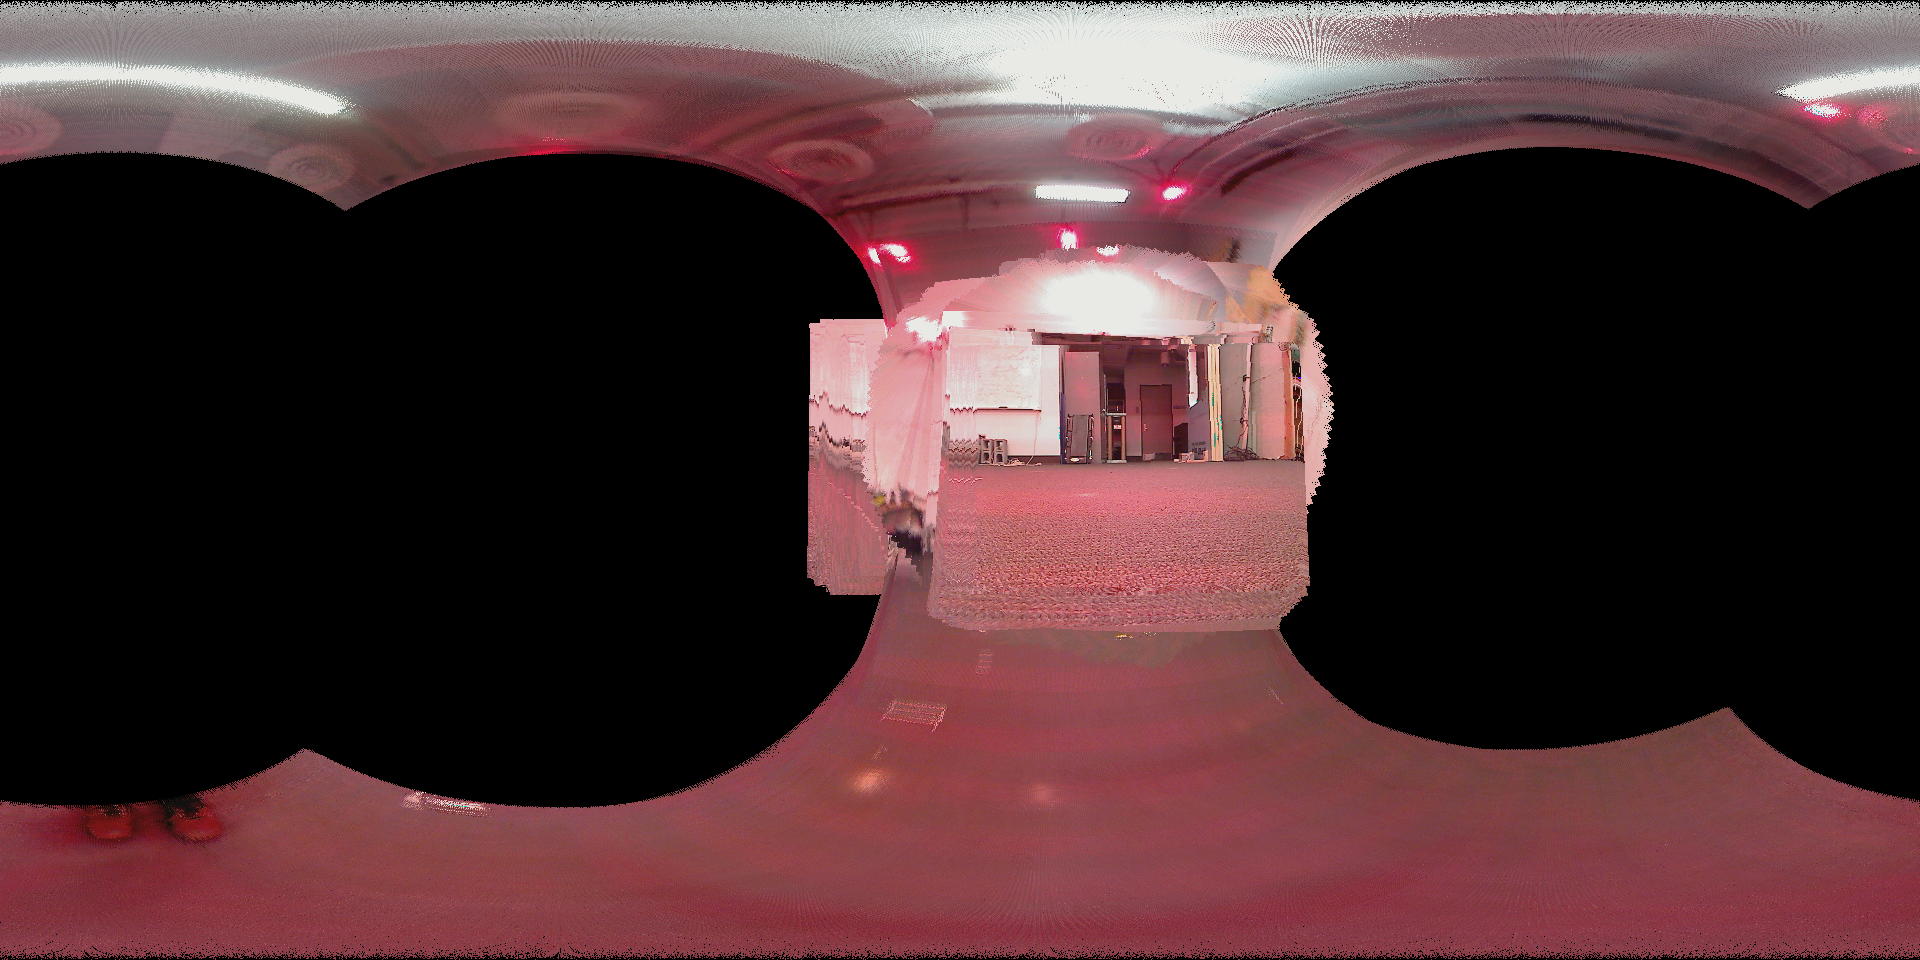
\includegraphics[width=2.5in]{../figs/panorama_1.png}
            % \caption{}
        \end{minipage}
    }%
    \centering
    \caption{ Result for Dataset 1}
\end{figure}

\begin{figure}[htbp]
    \centering
    \subfigure[Roll for Dataset 2]{
        \begin{minipage}[t]{1\linewidth}
            \centering
            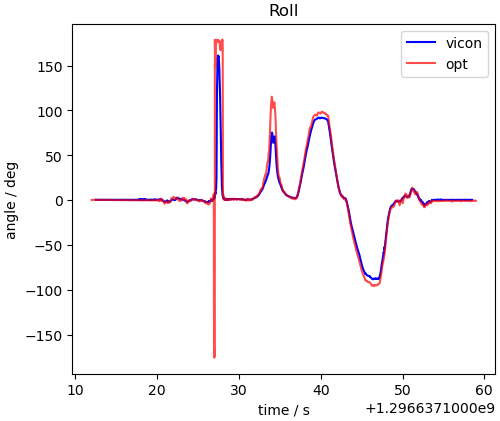
\includegraphics[width=2.5in]{../figs/Roll_2.png}
            % \caption{}
        \end{minipage}%
    }%

    \subfigure[Pitch for Dataset 2]{
        \begin{minipage}[t]{1\linewidth}
            \centering
            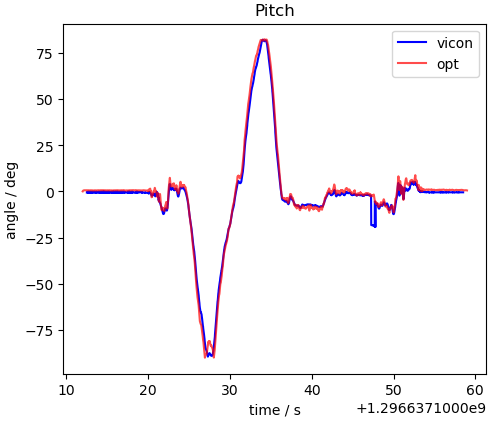
\includegraphics[width=2.5in]{../figs/Pitch_2.png}
            % \caption{}
        \end{minipage}
    }%

    \subfigure[Yaw for Dataset 2]{
        \begin{minipage}[t]{1\linewidth}
            \centering
            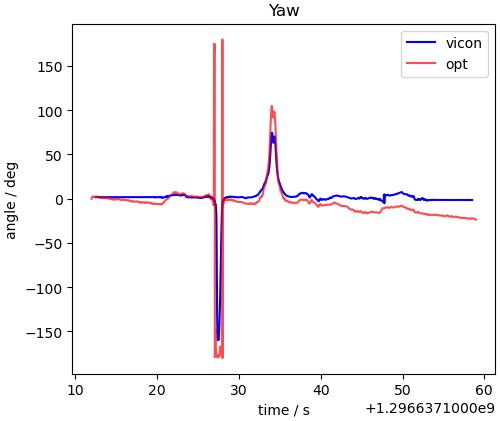
\includegraphics[width=2.5in]{../figs/Yaw_2.png}
            % \caption{}
        \end{minipage}
    }%

    \subfigure[Panorama for Dataset 2]{
        \begin{minipage}[t]{1\linewidth}
            \centering
            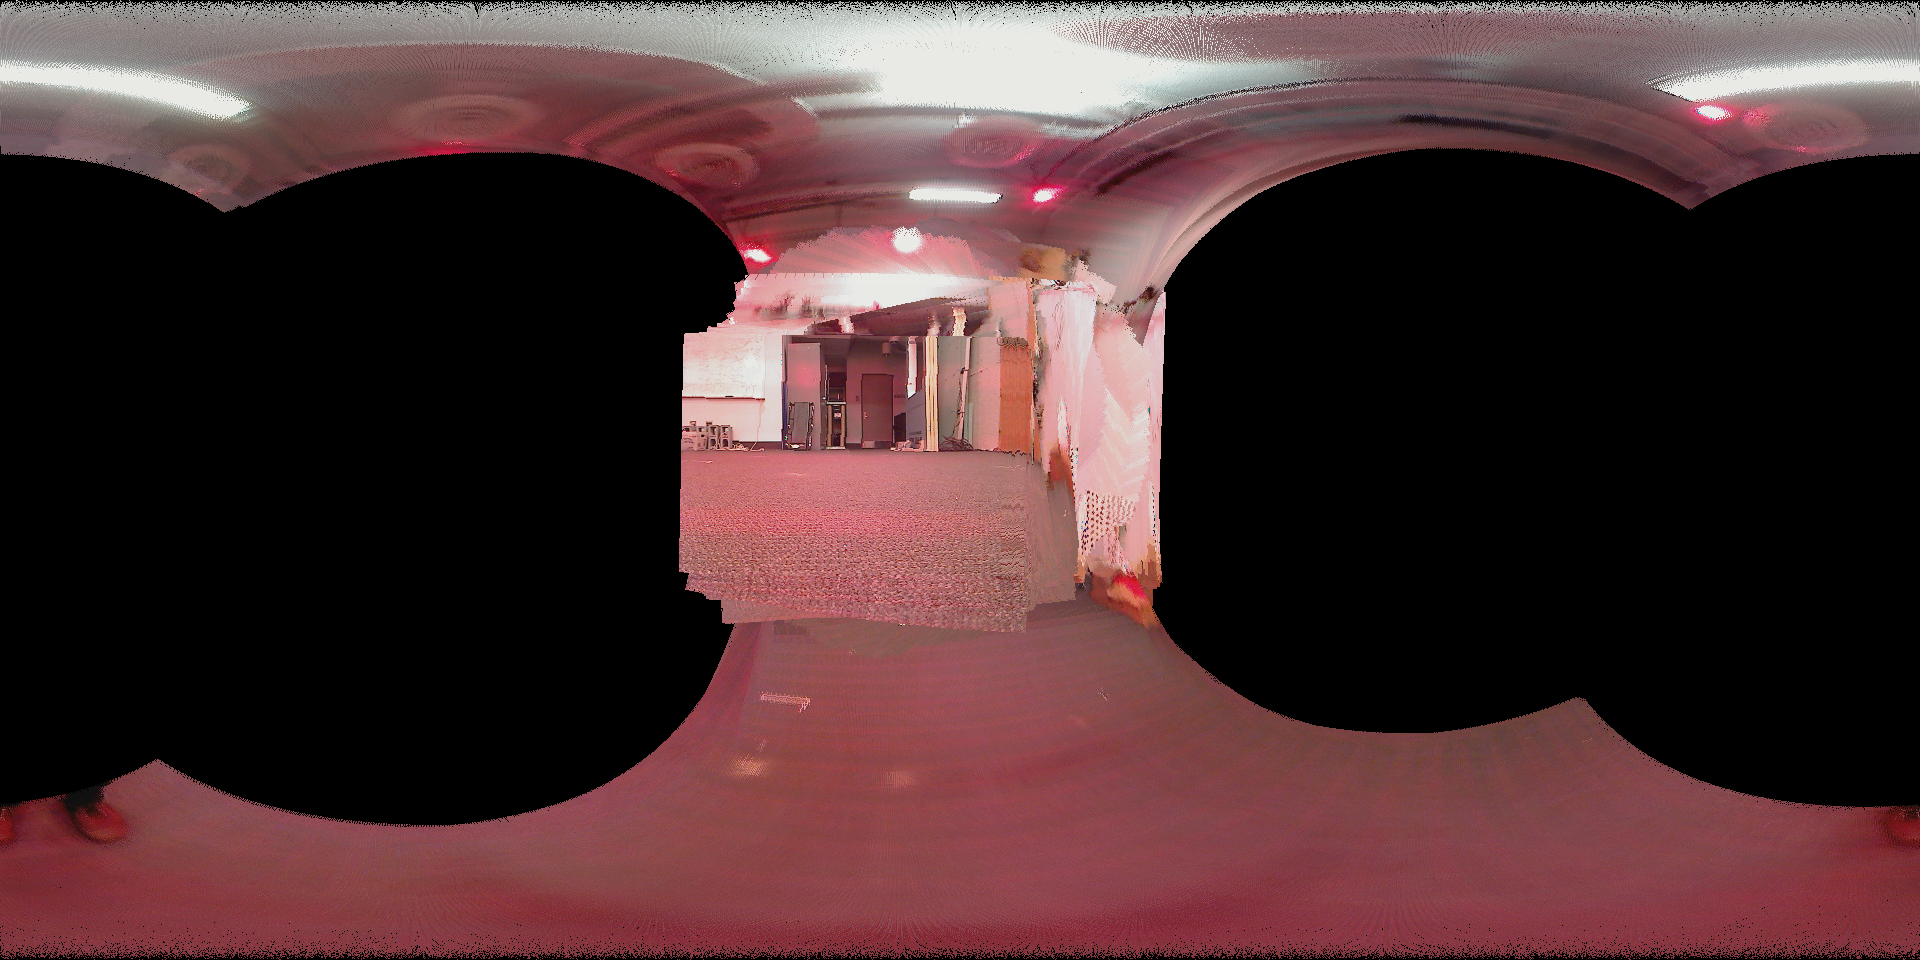
\includegraphics[width=2.5in]{../figs/panorama_2.png}
            % \caption{Panorama for Dataset 2}
        \end{minipage}
    }%
    \centering
    \caption{ Result for Dataset 2}
\end{figure}

\begin{figure}[htbp]
    \centering
    \subfigure[Roll for Dataset 3]{
        \begin{minipage}[t]{1\linewidth}
            \centering
            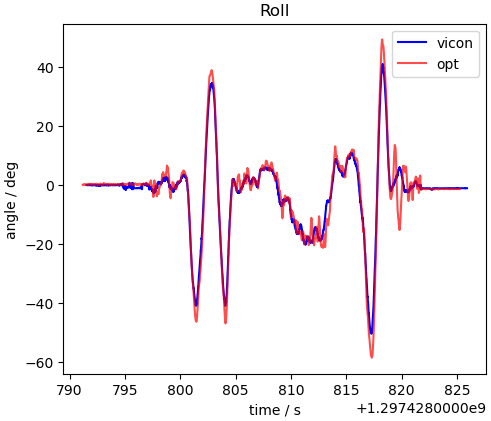
\includegraphics[width=2.5in]{../figs/Roll_3.png}
            % \caption{}
        \end{minipage}%
    }%

    \subfigure[Pitch for Dataset 3]{
        \begin{minipage}[t]{1\linewidth}
            \centering
            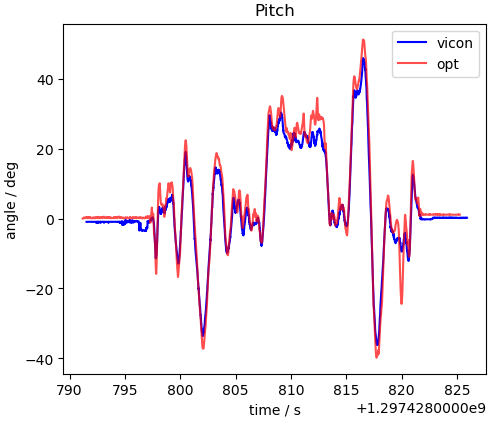
\includegraphics[width=2.5in]{../figs/Pitch_3.png}
            % \caption{}
        \end{minipage}
    }%

    \subfigure[Yaw for Dataset 3]{
        \begin{minipage}[t]{1\linewidth}
            \centering
            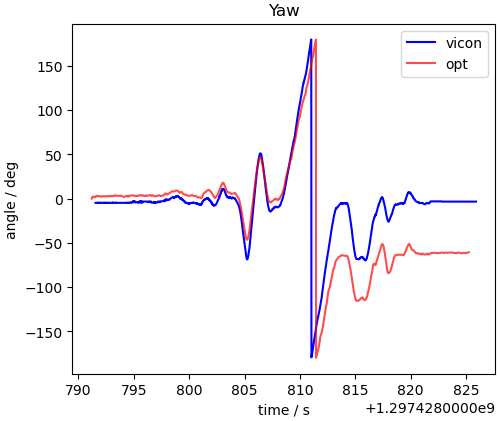
\includegraphics[width=2.5in]{../figs/Yaw_3.png}
            % \caption{}
        \end{minipage}
    }%

    \centering
    \caption{ Result for Dataset 3}
\end{figure}

\begin{figure}[htbp]
    \centering
    \subfigure[Roll for Dataset 4]{
        \begin{minipage}[t]{1\linewidth}
            \centering
            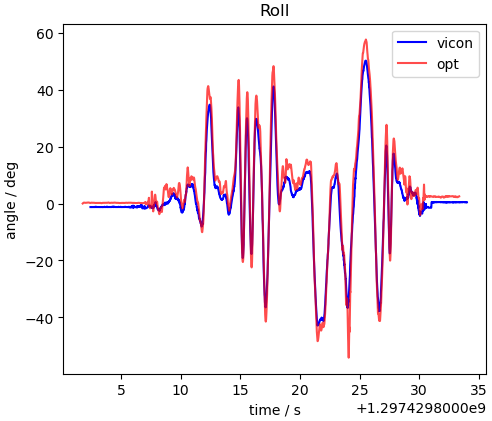
\includegraphics[width=2.5in]{../figs/Roll_4.png}
            % \caption{}
        \end{minipage}%
    }%

    \subfigure[Pitch for Dataset 4]{
        \begin{minipage}[t]{1\linewidth}
            \centering
            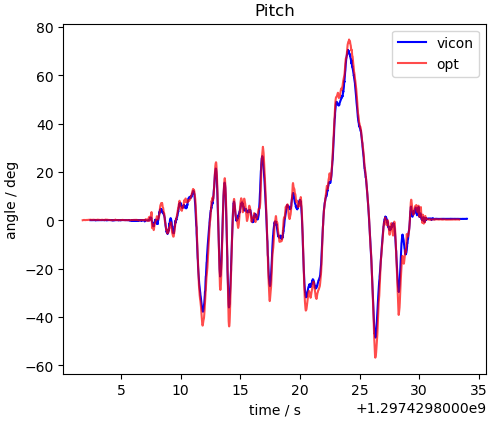
\includegraphics[width=2.5in]{../figs/Pitch_4.png}
            % \caption{}
        \end{minipage}
    }%

    \subfigure[Yaw for Dataset 4]{
        \begin{minipage}[t]{1\linewidth}
            \centering
            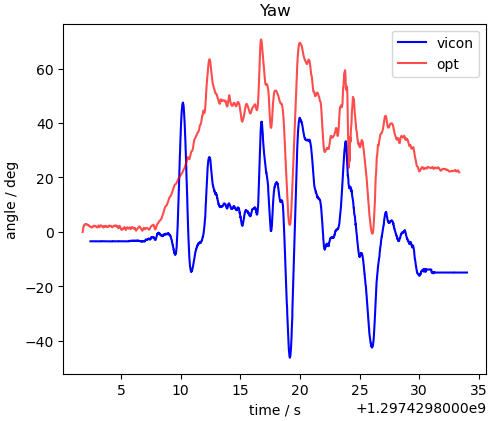
\includegraphics[width=2.5in]{../figs/Yaw_4.png}
            % \caption{}
        \end{minipage}
    }%
    \centering
    \caption{ Result for Dataset 4}
\end{figure}

\begin{figure}[htbp]
    \centering
    \subfigure[Roll for Dataset 5]{
        \begin{minipage}[t]{1\linewidth}
            \centering
            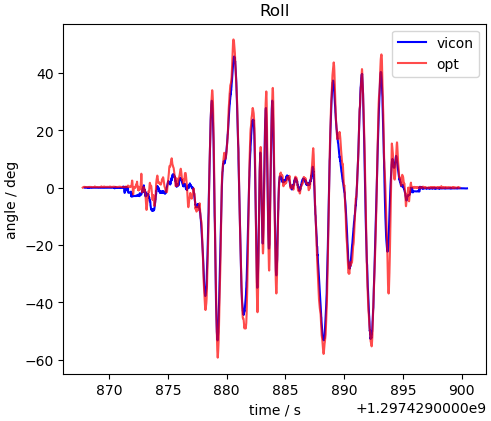
\includegraphics[width=2.5in]{../figs/Roll_5.png}
            % \caption{}
        \end{minipage}%
    }%

    \subfigure[Pitch for Dataset 5]{
        \begin{minipage}[t]{1\linewidth}
            \centering
            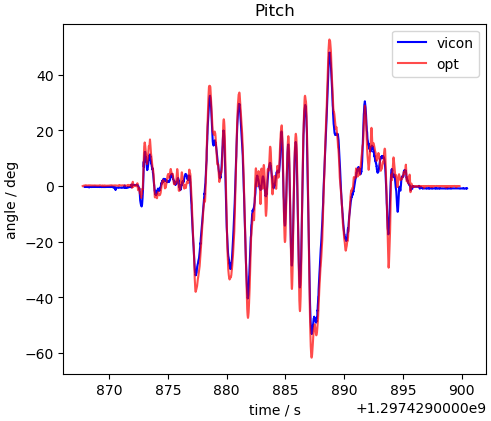
\includegraphics[width=2.5in]{../figs/Pitch_5.png}
            % \caption{}
        \end{minipage}
    }%

    \subfigure[Yaw for Dataset 5]{
        \begin{minipage}[t]{1\linewidth}
            \centering
            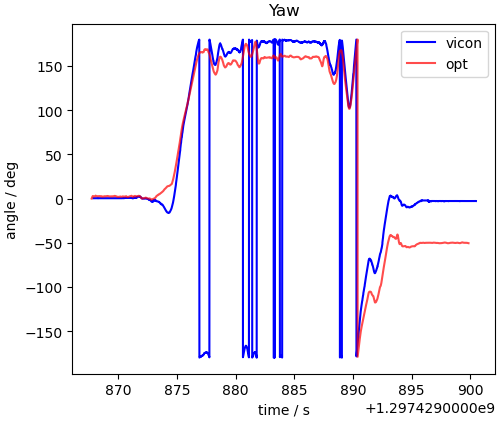
\includegraphics[width=2.5in]{../figs/Yaw_5.png}
            % \caption{}
        \end{minipage}
    }%

    \centering
    \caption{ Result for Dataset 5}
\end{figure}

\begin{figure}[htbp]
    \centering
    \subfigure[Roll for Dataset 6]{
        \begin{minipage}[t]{1\linewidth}
            \centering
            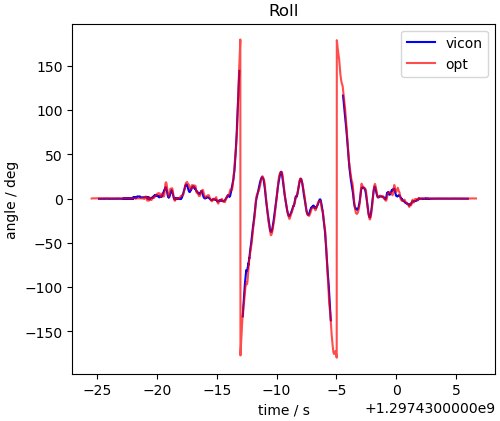
\includegraphics[width=2.5in]{../figs/Roll_6.png}
            % \caption{}
        \end{minipage}%
    }%

    \subfigure[Pitch for Dataset 6]{
        \begin{minipage}[t]{1\linewidth}
            \centering
            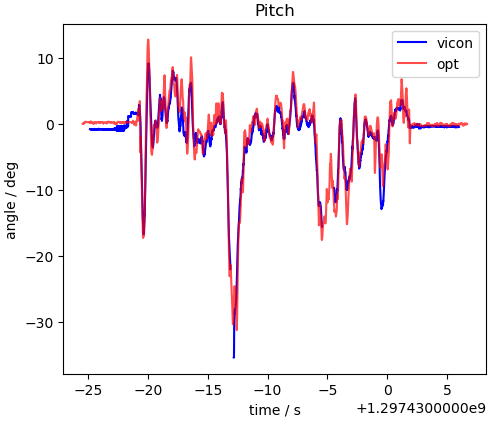
\includegraphics[width=2.5in]{../figs/Pitch_6.png}
            % \caption{}
        \end{minipage}
    }%

    \subfigure[Yaw for Dataset 6]{
        \begin{minipage}[t]{1\linewidth}
            \centering
            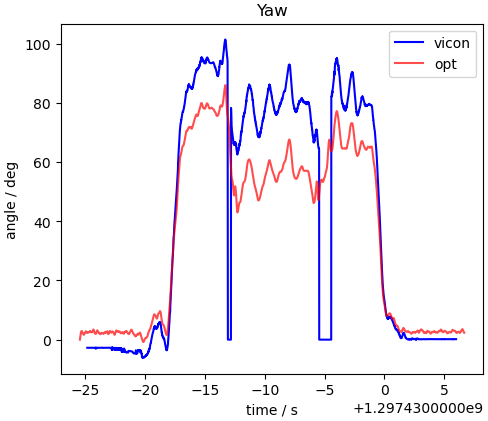
\includegraphics[width=2.5in]{../figs/Yaw_6.png}
            % \caption{}
        \end{minipage}
    }%

    \centering
    \caption{ Result for Dataset 6}
\end{figure}

\begin{figure}[htbp]
    \centering
    \subfigure[Roll for Dataset 7]{
        \begin{minipage}[t]{1\linewidth}
            \centering
            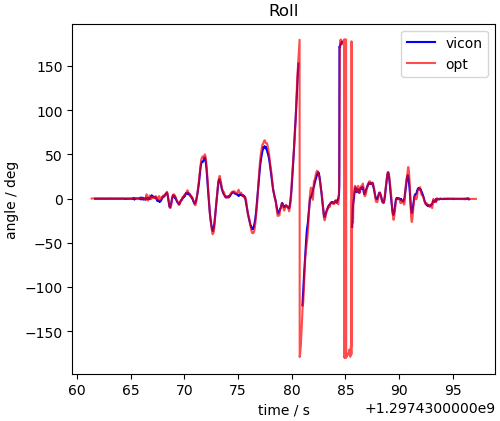
\includegraphics[width=2.5in]{../figs/Roll_7.png}
            % \caption{}
        \end{minipage}%
    }%

    \subfigure[Pitch for Dataset 7]{
        \begin{minipage}[t]{1\linewidth}
            \centering
            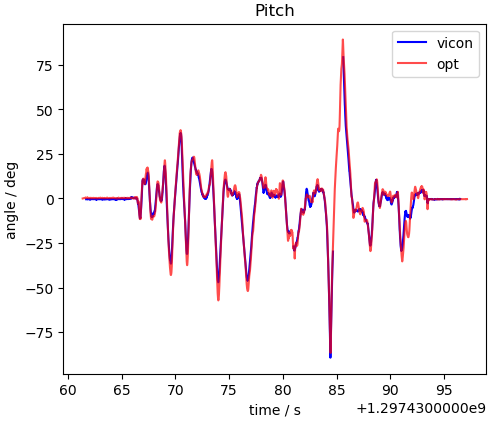
\includegraphics[width=2.5in]{../figs/Pitch_7.png}
            % \caption{}
        \end{minipage}
    }%

    \subfigure[Yaw for Dataset 7]{
        \begin{minipage}[t]{1\linewidth}
            \centering
            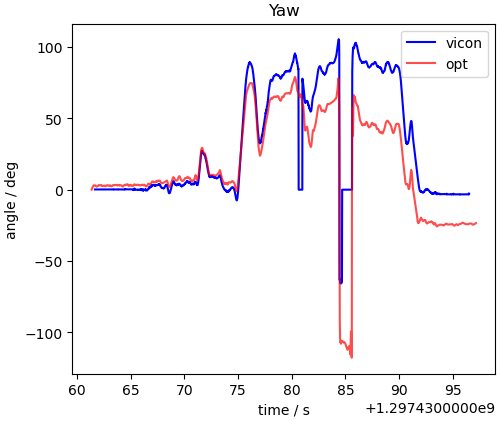
\includegraphics[width=2.5in]{../figs/Yaw_7.png}
            % \caption{}
        \end{minipage}
    }%

    \centering
    \caption{ Result for Dataset 2}
\end{figure}

\begin{figure}[htbp]
    \centering
    \subfigure[Roll for Dataset 8]{
        \begin{minipage}[t]{1\linewidth}
            \centering
            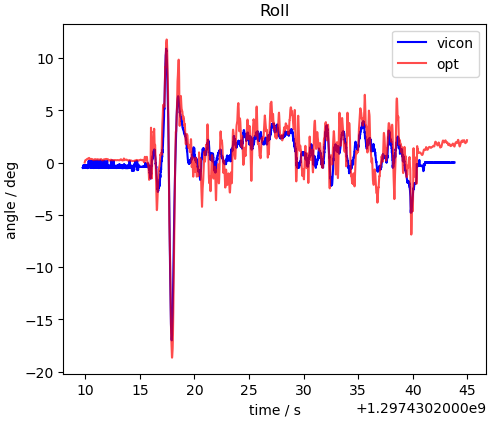
\includegraphics[width=2.5in]{../figs/Roll_8.png}
            % \caption{}
        \end{minipage}%
    }%

    \subfigure[Pitch for Dataset 8]{
        \begin{minipage}[t]{1\linewidth}
            \centering
            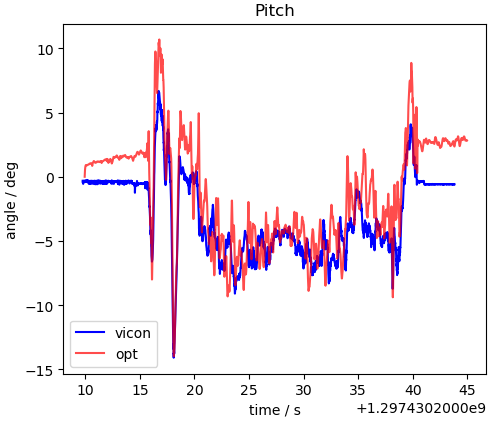
\includegraphics[width=2.5in]{../figs/Pitch_8.png}
            % \caption{}
        \end{minipage}
    }%

    \subfigure[Yaw for Dataset 8]{
        \begin{minipage}[t]{1\linewidth}
            \centering
            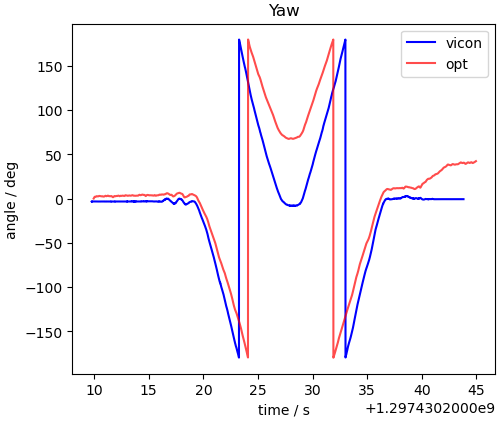
\includegraphics[width=2.5in]{../figs/Yaw_8.png}
            % \caption{}
        \end{minipage}
    }%

    \subfigure[Panorama for Dataset 8]{
        \begin{minipage}[t]{1\linewidth}
            \centering
            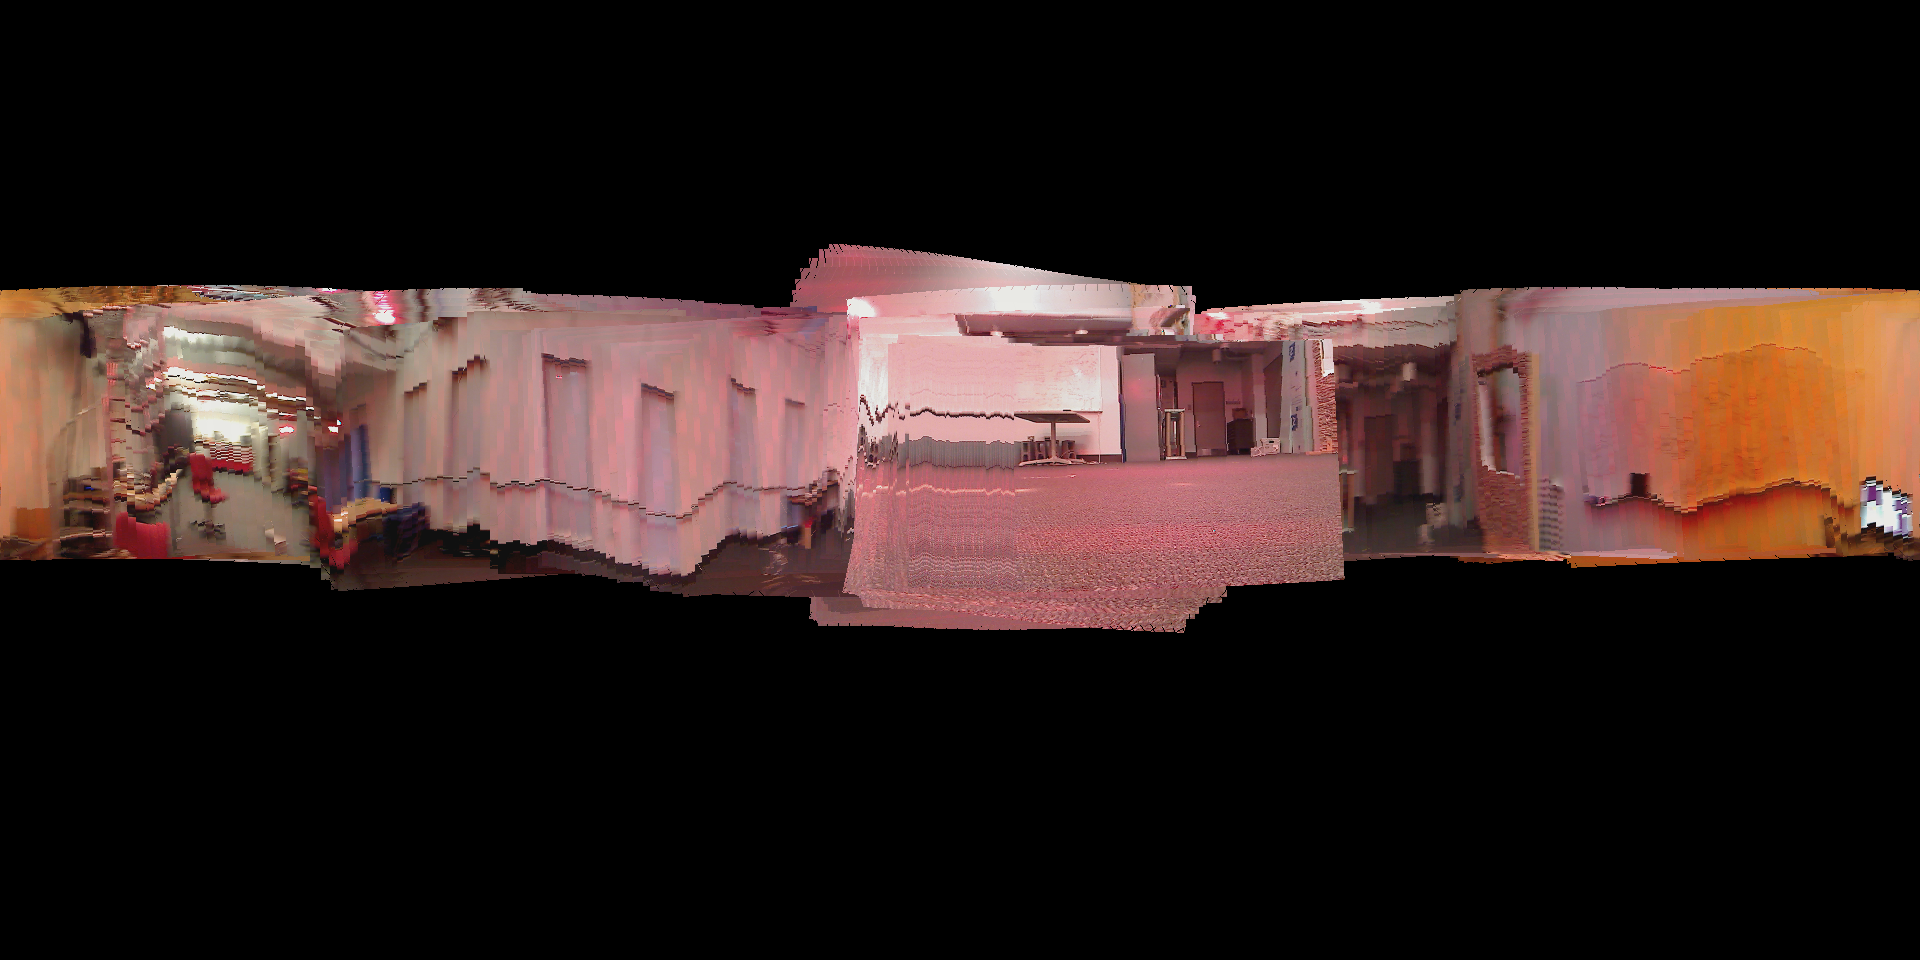
\includegraphics[width=2.5in]{../figs/panorama_8.png}
            % \caption{Panorama for Dataset 2}
        \end{minipage}
    }%
    \centering
    \caption{ Result for Dataset 8}
\end{figure}

\begin{figure}[htbp]
    \centering
    \subfigure[Roll for Dataset 9]{
        \begin{minipage}[t]{1\linewidth}
            \centering
            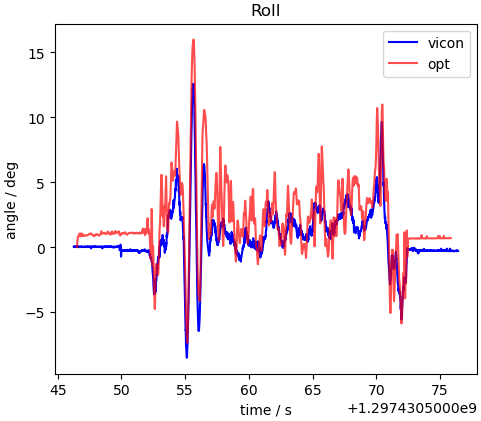
\includegraphics[width=2.5in]{../figs/Roll_9.png}
            % \caption{}
        \end{minipage}%
    }%

    \subfigure[Pitch for Dataset 9]{
        \begin{minipage}[t]{1\linewidth}
            \centering
            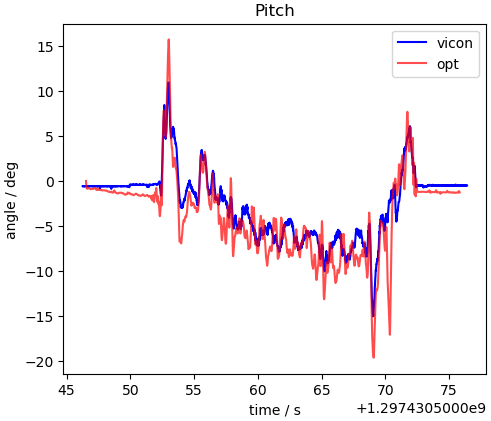
\includegraphics[width=2.5in]{../figs/Pitch_9.png}
            % \caption{}
        \end{minipage}
    }%

    \subfigure[Yaw for Dataset 9]{
        \begin{minipage}[t]{1\linewidth}
            \centering
            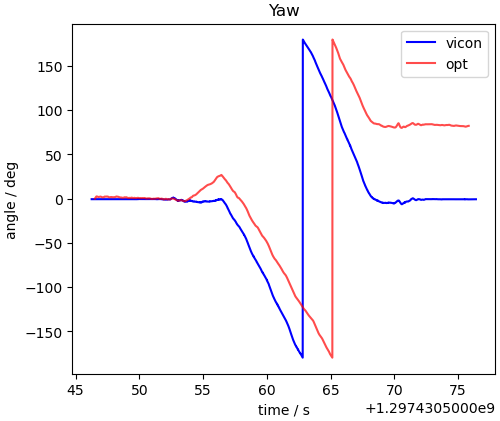
\includegraphics[width=2.5in]{../figs/Yaw_9.png}
            % \caption{}
        \end{minipage}
    }%

    \subfigure[Panorama for Dataset 9]{
        \begin{minipage}[t]{1\linewidth}
            \centering
            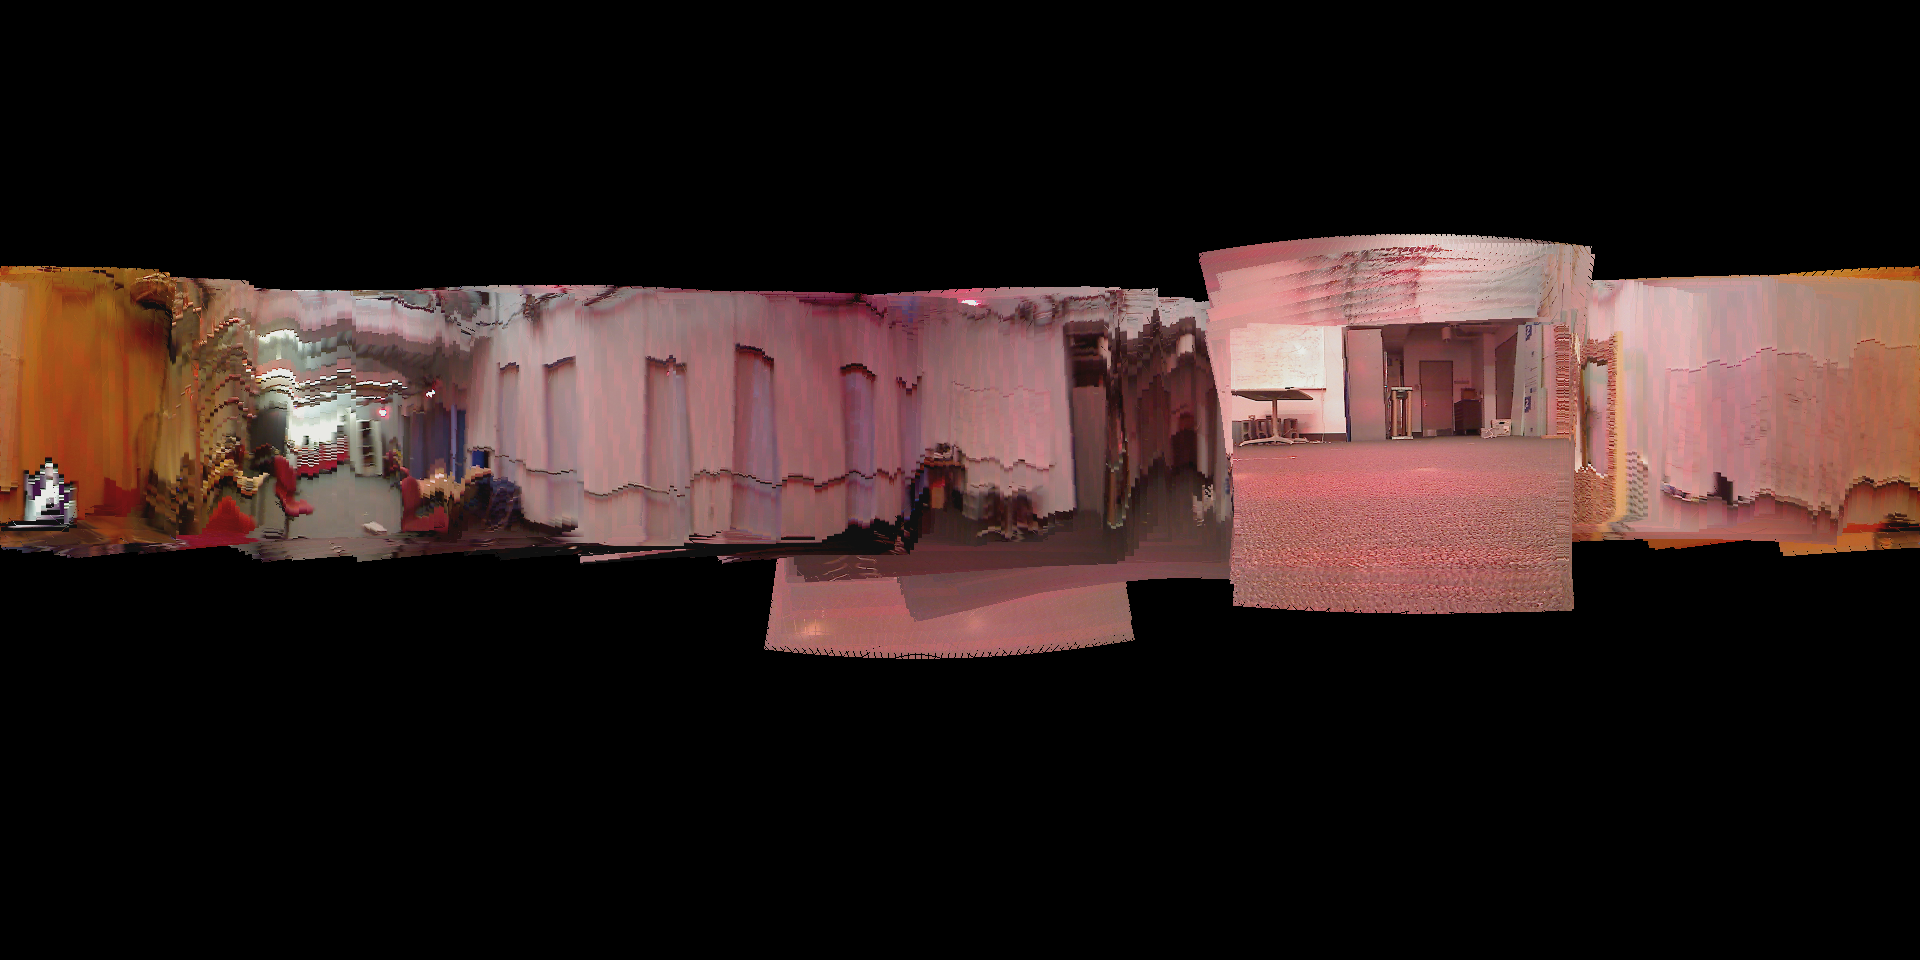
\includegraphics[width=2.5in]{../figs/panorama_9.png}
            % \caption{Panorama for Dataset 2}
        \end{minipage}
    }%
    \centering
    \caption{ Result for Dataset 9}
\end{figure}

\begin{figure}[htbp]
    \centering
    \subfigure[Roll for Dataset 10]{
        \begin{minipage}[t]{1\linewidth}
            \centering
            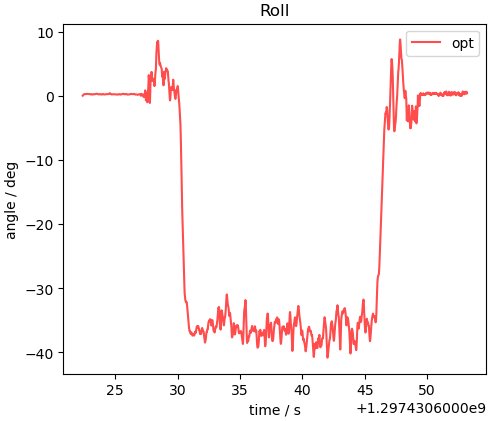
\includegraphics[width=2.5in]{../figs/Roll_10.png}
            % \caption{}
        \end{minipage}%
    }%

    \subfigure[Pitch for Dataset 10]{
        \begin{minipage}[t]{1\linewidth}
            \centering
            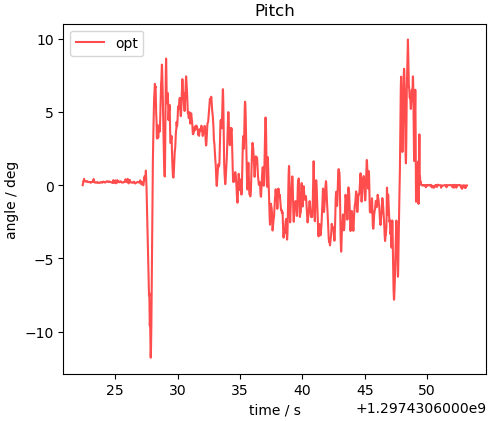
\includegraphics[width=2.5in]{../figs/Pitch_10.png}
            % \caption{}
        \end{minipage}
    }%

    \subfigure[Yaw for Dataset 10]{
        \begin{minipage}[t]{1\linewidth}
            \centering
            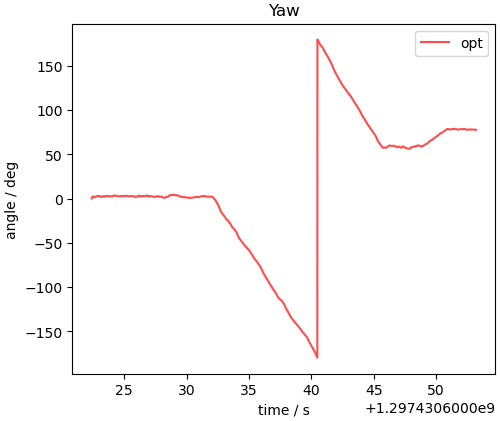
\includegraphics[width=2.5in]{../figs/Yaw_10.png}
            % \caption{}
        \end{minipage}
    }%

    \subfigure[Panorama for Dataset 10]{
        \begin{minipage}[t]{1\linewidth}
            \centering
            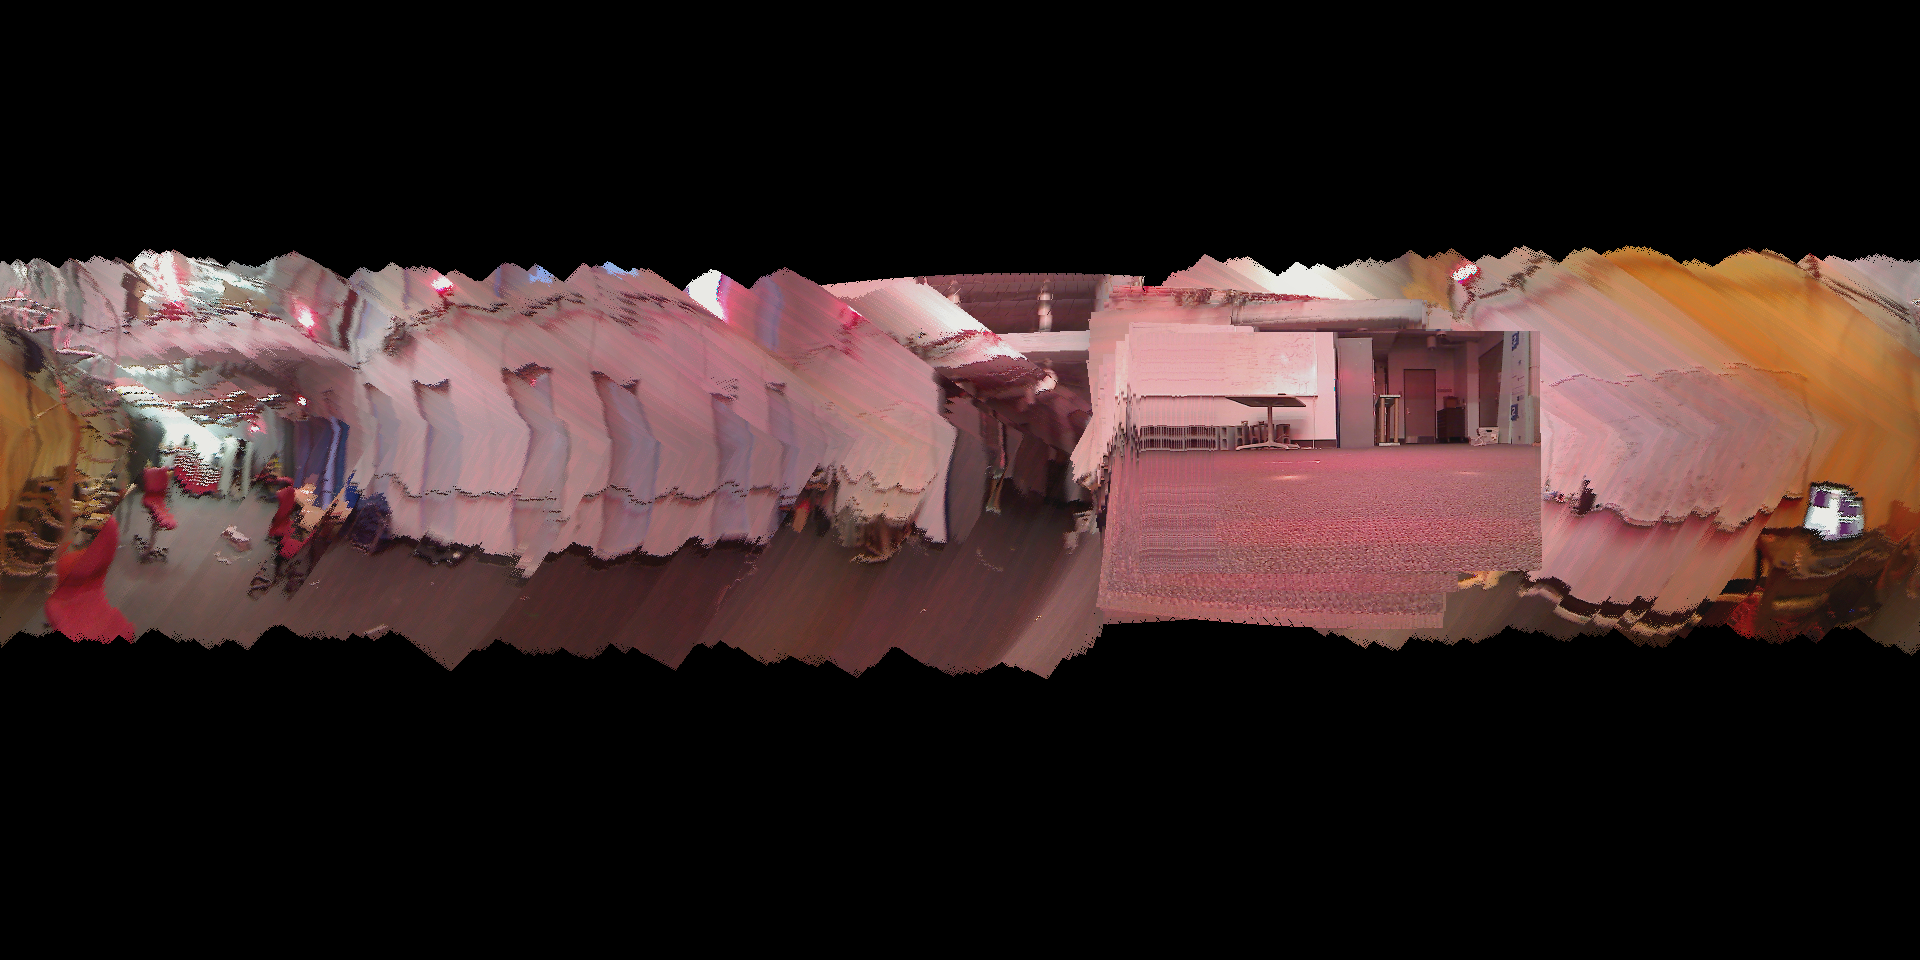
\includegraphics[width=2.5in]{../figs/panorama_10.png}
            % \caption{Panorama for Dataset 2}
        \end{minipage}
    }%
    \centering
    \caption{ Result for Dataset 10}
\end{figure}

\begin{figure}[htbp]
    \centering
    \subfigure[Roll for Dataset 11]{
        \begin{minipage}[t]{1\linewidth}
            \centering
            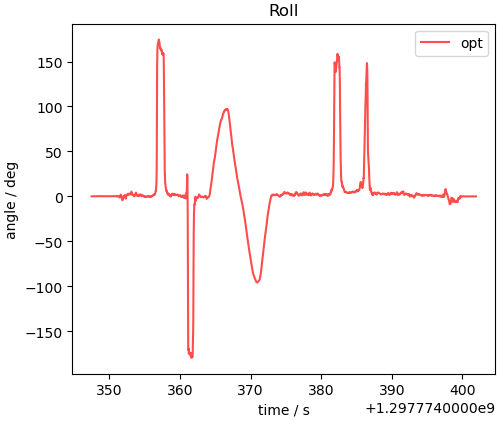
\includegraphics[width=2.5in]{../figs/Roll_11.png}
            % \caption{}
        \end{minipage}%
    }%

    \subfigure[Pitch for Dataset 11]{
        \begin{minipage}[t]{1\linewidth}
            \centering
            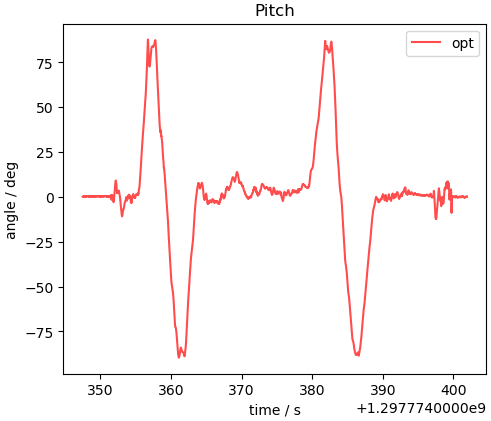
\includegraphics[width=2.5in]{../figs/Pitch_11.png}
            % \caption{}
        \end{minipage}
    }%

    \subfigure[Yaw for Dataset 11]{
        \begin{minipage}[t]{1\linewidth}
            \centering
            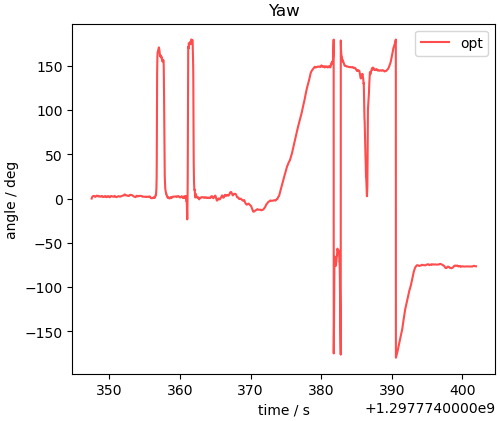
\includegraphics[width=2.5in]{../figs/Yaw_11.png}
            % \caption{}
        \end{minipage}
    }%

    \subfigure[Panorama for Dataset 11]{
        \begin{minipage}[t]{1\linewidth}
            \centering
            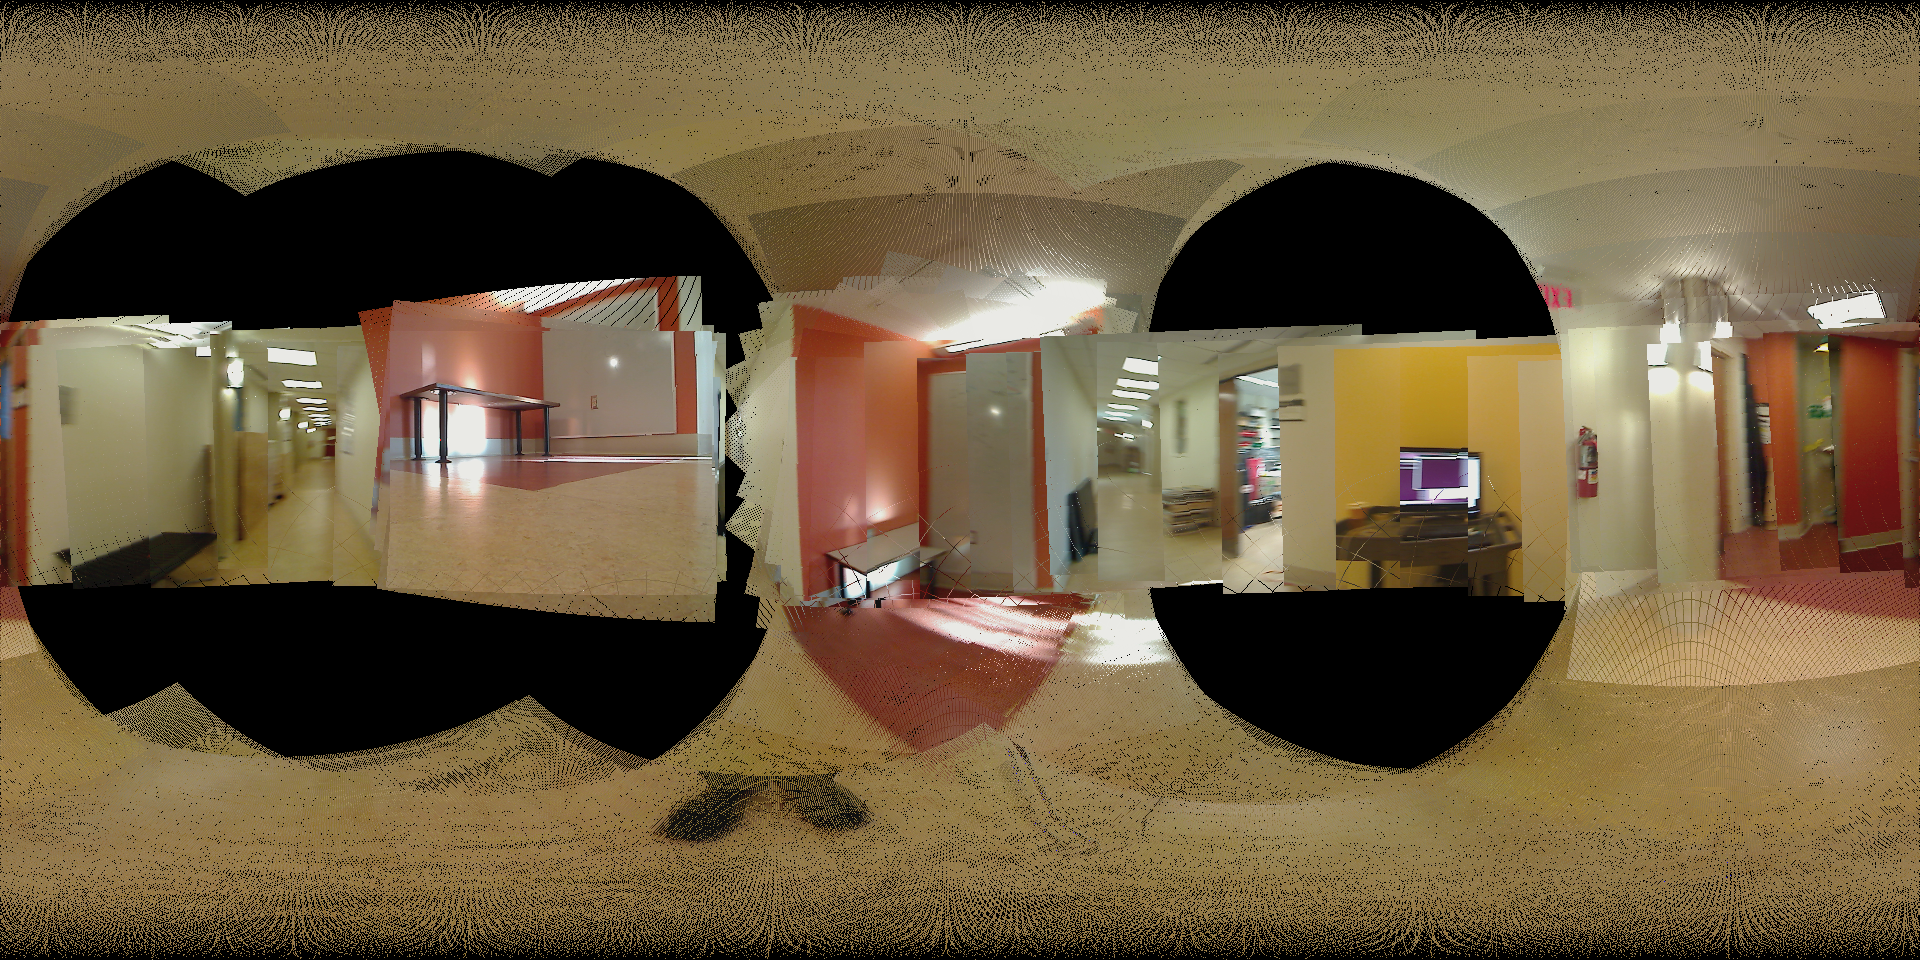
\includegraphics[width=2.5in]{../figs/panorama_11.png}
            % \caption{Panorama for Dataset 2}
        \end{minipage}
    }%
    \centering
    \caption{ Result for Dataset 11}
\end{figure}

\end{document}
